\documentclass[12pt]{article}

\usepackage{amsmath, amssymb, amsthm, graphicx, fancyhdr, textcomp, enumerate, diagbox, tcolorbox, esvect, tikz, adjustbox}

\graphicspath{{./images/}}

\usepackage{halloweenmath, tikzsymbols}

\newcommand{\R}{\mathbb{R}}
\newcommand{\Z}{\mathbb{Z}}
\newcommand{\C}{\mathbb{C}}
\newcommand{\N}{\mathbb{N}}
\newcommand{\Q}{\mathbb{Q}}
\newcommand{\Arg}{\mbox{Arg}}
\newcommand{\Log}{\mbox{Log}}

%geometry/topology
\newcommand{\bndry}{\partial}


\newcommand{\infsum}{\sum_{n = 1}^{\infty}}
\newcommand{\pf}{\fbox{proof}}
\newcommand{\cor}{\fbox{corollary}}

\theoremstyle{definition}

\newtheorem*{definition}{Definition}
\newtheorem{lemma}{Lemma}
\newtheorem{theorem}{Theorem}
\newtheorem{corollary}{Corollary}
\newtheorem{proposition}{Proposition}
\newtheorem{remark}{Remark}
\newtheorem{conjecture}{Conjecture}
\newtheorem{example}{Example}

\newcommand{\inv}[1]{#1^{-1}}

\title{Modern Geometry}
\author{August}

\begin{document}

\maketitle

\section{Problem 6.17}

Compute the Euler Characteristic and genus for these polyhedra:

\includegraphics[scale=0.25]{Figure6-10.png} 

For (a), I'll compute the Euler charactaristic directly (vertices minus edges plus faces), and compute the genus from that. Since just by looking at the shape we can see that it has genus three, I'll use that and show that the Euler charactaristic matches up.

Counting the number of faces, we find that there are $F = 3(4) + 3 + 4(3) = 27$ faces (the square faces plus the  rising faces plus the tube faces).

Now for the edges, we have the normal twelve of the cube, as well as twelve of the "rising" edges to the "tubes" as well as those of the tubes, we have $E = 12 + 12 + 4(3) + 4(3) + 7 = 55$ edges.

Now for the vertices, we have eight of the cube vertices, as well as twelve of the tube endings, as well as four at the intersection of the tubes, in total $V = 8 + 12 + 6 = 26$ vertices.

Now applying Euler's formula we have $\chi(S) = V - E + F = 26 - 46 + 27 = -2$. Solving the formula given to use by the textbook (Theorem 6.15) we find that the genus is $g = 2$. This tells us that, roughly speaking, this polyhedron is a doughnut with two holes. That's not obvious just by looking at it.

Now for (b), there are $V = 4(6) + 6 = 30$ vertices. There are $F = 2( 4(2) + 1 + 4) + 2(4) + 2(4) = 42$, and there are $E = 8(2) + 4(6) + 4(2) + 8 + 8 + 4 = 68$ edges. Therefore the Euler characteristic is $\chi(S) = V - E + F = 30 - 84 + 42 = -12$.

From this we can compute the genus, using the formula $\chi(S) = -12 = 2 - 2g$. Solving the equation, we have $g = 7$.

\begin{remark}
Computing the genus in this was is actually somewhat surprising. 
\end{remark} 


\section{Problem 6.46}


\includegraphics[scale=0.5]{unfolding_proof.png}


\begin{proposition}

The above polyhedron does not have a net.
\end{proposition}


\begin{proof}

The faces $A$ and $C$ (where $C$ is the face opposite $A$) must be connected in any net, by a string of adjacent edges. Each such path will cross through an face of the form $B$ (one of the non-convex ones which is adjacent to $A$. Therefore, one of the edges of the form $a$, $b$, or $c$ must not be "cut" in a net. We rule out each of these possibilities, thereby proving this polyhedron does not have a net.

\begin{itemize}
\item[$a$] Here we note that, in order to keep the face $B$ congruent in the net, we must have the other edge of $a$ also adjacent. The square faces of the form $Z$, $X$, and $Y$ must also lie flat in the plane. If we regard the area of one of the square faces as $1$, we note that in total, all four of the square faces will have an area of $4$. Connecting $A$ and $B$ at $a$ demands that this area of $4$ fit in the open space left by $A$ and $B$, as shown in the figure. This has area $2$, so it impossible to "unwrap" the square faces. Hence the case where $a$ is connected is ruled out.

\includegraphics[scale=1]{unfolded_a.png} 

\item[$c$] Now suppose that the path of adjacent edges in the supposed net crosses through $c$. This won't work either, because we will have to "fold $Y$ along $c$ towards the opposite side, closing in the concave square bit of $A$. This leaves no room for $X$ to be unfolded.

\item[$b$] finally, suppose we connect $A$ to $B$ through $b$. If we do this, we will have to fold $X$ along $b$ away from $A$, and either connect to $Y$ or $Z$ ($Y$ is of course considered up to symmetry, since we could have tried and connected along the one opposite $Y$ as well). If we connect along $Z$, we will necessarily make $A$ and $B$ adjacent through $a$ adjacent (even if it is cut), and we once again have the problem of unfolding four equal sized squares into an area of only two of the squares. Now if we connect $X$ to $Y$ to $B$, we will end up having to cover over the face $Z$ with $B$, as shown in the figure:

\includegraphics[scale=1]{unfold_along_Z.png} 

\end{itemize}

As we can see, no possible cases work, so we cannot have a net of the polyhedron. 
\end{proof}

\section{Problem 6.59}

Here is the star unfolding for the tetrahedron centred at the vertex labelled 1. Obviously, the cuts are in red. 

\includegraphics[scale=0.5]{tetrahedron_unfolding.png}

Note that the irregularity of the triangles is only because of Geogebra. Note also the amount of symmetry to this unfolding: it is the same as that of the triangle. 

Now for the star unfolding of the octahedron:

\includegraphics[scale=0.5]{octahedron_unfolding.png} 

This is less symmetric, but it still does have four symmetries. The cube is not so lucky. Once again, the star unfolding is centred at the vertex labelled 1.

Finally, for the cube, this is the star unfolding:

\includegraphics[scale=0.5]{cube_unfolding.png} 

Interestingly, the cube doesn't have any symmetries at all. I think the amount of symmetry has to do with the length of the maximal minimal path from $1$ to another vertex. I also think the tetrahedron is the only case that gives us a net, since in order to not cut through the faces, we would have to have every vertex connected to every vertex by one edge, and this would immediately turn our polyhedron into a tetrahedron.



\section{Problem (c)}

\begin{proposition} Let $P_{1,2,3,4}$ be convex polygons. Suppose that the intersection of any three of them is non-empty. Then the intersection of all four of them is non-empty.
\end{proposition}

This is obviously false about sets in general, and with a bit of work it is possible to find a counterexample with non-convex polygons. Hence we need them to be convex. However, I don't think we need them to be polygons. My proof works for convex sets in general. Note that we have shown that a polygon is a convex region if and only it's vertices are convex. I am taking it for granted that convex polygons are convex.

\begin{proof}

Since the intersection of any three of them is non-empty, we have points $p_{2,3,4}, p_{1,3,4}, p_{1,2,4}, p_{1,2,3} $ in each intersection respectively (as in, $p_{ijk}\in P_{i}\cap P_{j} \cap P_{k}$ .\\

There are four cases as to the shape of the convex hull of these four points. The first case is that the convex hull is a single point. In this case, this point is in all of them, and we're done.\\

If the convex hull is a line, then one point is between the rest, and therefore is in all of them by convexity. \\

If the convex hull is a triangle, without loss of generality suppose that $p_{123}$ is in the interior of the convex hull, while the vertex points all are contained within $P_4$. Well then, in this case convexness of $P_4$ requires that the triangle formed by the other four points is contained within $P_4$, and as a consequence, so is $p_{123}$. Since by construction of $p_{123}$, the point is in $P_1$, $P_2$, and $P_3$, it follows that the point $P_{123}$ is contained within all four of the polygons as desired. Hence the intersection of all four polygons is non-empty.

Now for the case where the convex hull of these points is a convex quadrilateral. It is true that the diagonals of a convex quadrilateral meet at a point, call it $p$. I claim that this point is contained within all four polygons. Without loss of generality (labelling was arbitrary, and could just as well have been permuted in any way we liked), suppose that the convex polygon which is the convex hull of the four points, has vertices written in cyclic order: $ p_{234}p_{134}p_{124}p_{123}. $ The diagonals are the non-adjacent pairs, which in this case are $ p_{234}p_{124} $ and $ p_{134}p_{123}$. Then the intersection of these diagonals, by construction, is $p$. Now we aim to show that $p\in P_1\cap ...\cap P_4$. Since $p$ is on the line segment $p_{234}p_{124}$, and since both of these points are in the polygons $P_2$ and $P_4$, both of which are convex (and hence by convexness the line segment between them is contained within both of them), we have that $p\in P_2,P_4$. By an identical argument in the case of the segment $p_{134}p_{123}$ with the polygons $P_1$ and $P_3$, we find that $p\in P_1, P_3$. So $p\in P_1\cap ... \cap P_4$ as desired.\\

Since the convex hull of four points can be either a point, a line, a triangle, or a convex quadrilateral, we have covered every possibility. This concludes the proof.
\end{proof}


\section{Problem (a)}

\begin{proposition}
For all pairs of integers $(v,f)$ satisfying $v\le 2f-4$ and $f\le 2v-4 $, there exists a polyhedron with $v$ vertices and $f$ faces.
\end{proposition}

My proof will be by induction. For the purpose of making my proof more elegant, I'll start by providing a couple of lemmas, and doing the dirty work of manipulating the inequalities. Then I'll jump into the actual proof.

First, we must have $v\ge 4$ and $f\ge 4$, for these are the vertices and edges of polyhedra. A polyhedron with only three vertices must, by any reasonable axiom of geometry, lie in a plane. We don't want to call this a polyhedron. So $v \ge 4$. Moreover, the first inequality gives us that $ 4\le v \le 2f-4 $ hence $ 4\le 2f-4$ hence $8 \le 2f$ so $ 4 \le f $. This establishes that both $v$ and $f$ must not be less than $4$ (of course, negative or zero number of vertices would make even less sense).

Now I'll outline three methods of appending vertices to polyhedra, in which the number of faces added is either $2$ and $1$, and so that, given a polyhedron, it is also possible to append one vertex while adding whichever of these numbers of faces we happen to feel like adding.

\begin{lemma}
Given a polyhedron $P$, it is always possible to construct a polyhedron $P'$ with one more vertex and one more face than $P$. Moreover, it is also always possible to construct a polyhedron with one more vertex, and two more faces.
\end{lemma}

\begin{proof}

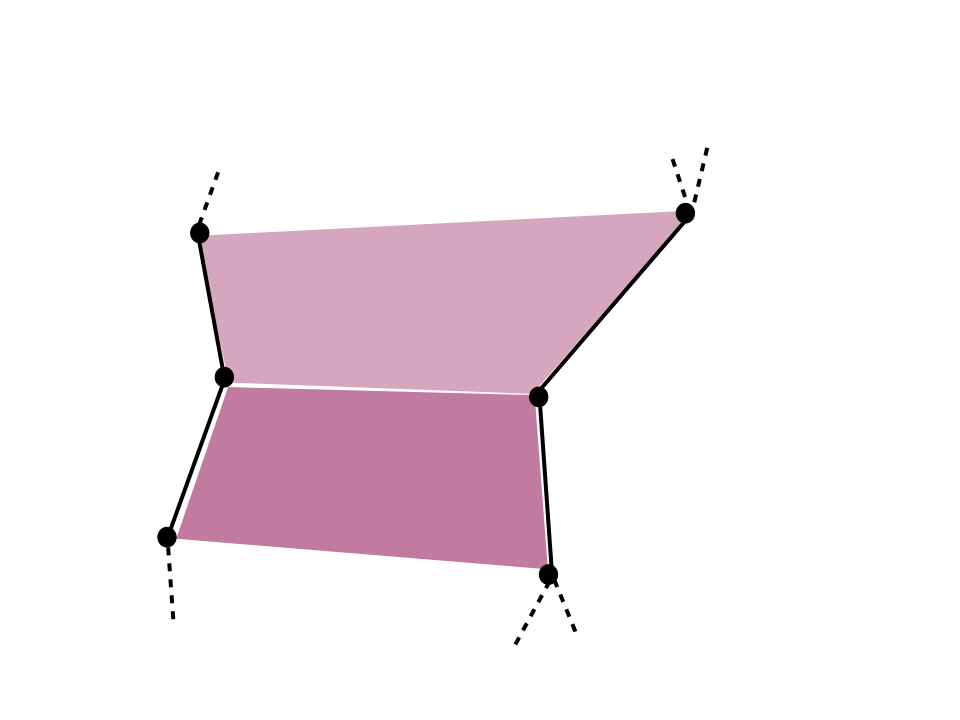
\includegraphics[scale=0.5]{General Polyhedron edge (1).jpg} 

I'll outline two generic constructions which are always possible to carry out, each of which results in a polyhedron with exactly one more vertex. Then I'll show that for any polyhedron, it is always possible to chose one of these constructions to get either of $1$ or $2$ (I mean whichever we like, not "or" as we usually mean it).

\includegraphics[scale=0.5]{V1.jpg} 

The first I call $V2$. The idea is to append a new vertex on the polygon $F3$, and to form a new face $U$ as shown in the figure. This adds exactly one face with one new vertex.

\includegraphics[scale=0.5]{V2.jpg} 

I call this one $V2$, and it is similar, but we also add a new face $V$ as well as $U$, as shown in the figure. The resulting polyhedron will have two more faces, and one more vertex.

It is always possible to carry out these constructions on a polygon. Therefore, given a polyhedron with $v$ vertices and $f$ faces, we can construct a new polyhedron with $v+1$ vertices and $f + 1$ faces, as well sa one with $v+1$ vertices and $f+2$ faces.

Now we can forget about these constructions for the actual proof, keeping only the fact that we can always add one or two faces by adding one vertex. 


\end{proof}

Now we can actually proceed to the proof of the lemma.

\begin{proof}
The proof is by induction. The base case is where $v = 4$, so $f = 4$, and we have the tetrahedron. \\

Now suppose that for all numbers of faces $f$ for which the inequalities hold with $n$ vertices, we have an associated polyhedron with $n$ vertices and $f$ faces. This is our induction assumption.

We now consider the number $n+1$. Notice that the inequality $v \le 2f - 4$ demands that $v/2 + 2 \le f$, so we have a lower bound for $f$ in terms of $v$. If we add one new vertex, we have $ (n + 1)/2 + 2 $ as our new lower bound. By the induction assumption ceiling function of $n/2 + 2$ must have had some polyhedron associated with it, and the ceiling function of $(n+1)/2 + 2$ exceeds that of $n/2 + 1$ by no more than $1$. We can add one face by the previous lemma, as well as all the way up to one less than our previous upper bound of $2n -4$. But notice that our new upper bound is $2n - 2$ (adding one vertex), so in order to get the last associated $f$ to have a polyhedron, we must add two faces by adding only one vertex to the polyhedron with $2n - 2$ faces (which was provided by our induction assumption). By the previous lemma, we can do this as well. So the induction step holds.

This completes the proof. 
\end{proof}

\section{Problem 7.4}

Here I construct a class of environments with $\Omega(n^2)$ path components, where $n$ is the number of vertices. Each member of this class of environments with $n$ vertices will have $2n-2$ path components.

For the base case, consider the below configuration of points, with the ladder labelled in magenta. You may not agree (though you should) that there are no more than one path component, but you will no doubt agree that there is at least one :).

\includegraphics[scale=0.5]{Base Case.jpg} 




\end{document}
